\chapter{Introduzione alla Mixed Reality}

\section{Cenni Storici}\label{sec:Sezione1.1}
I concetti di realtà virtuale (VR) e realtà aumentata (AR) comparirono per la prima volta nel 1965, quando Ivan Sutherland (ricercatore dell’Università di Harvard) pubblicò un saggio \cite{theultimatedisplay} contenente la seguente citazione:
\begin{center}
\textit{“The ultimate display would, of course, be a room within which the computer can control the existence of matter. A chair displayed in such a room would be good enough to sit in. Handcuffs displayed in such a room would be confining, and a bullet displayed in such a room would be fatal. With appropriate programming such a display could literally be the Wonderland into which Alice walked.”} 
\end{center}

\begin{figure}[t]
    \centering
    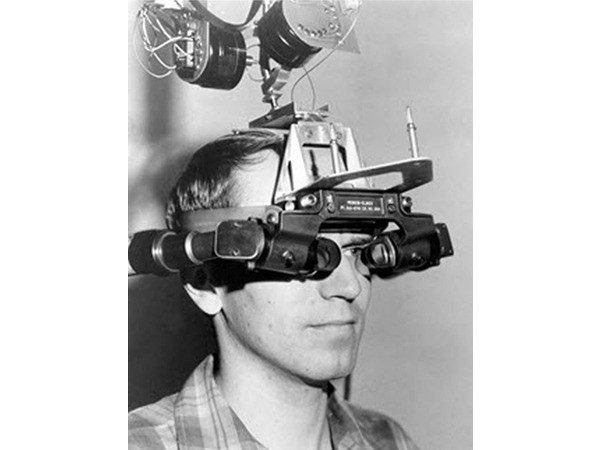
\includegraphics[width=\textwidth]{images/sword-of-damocles-vr.jpg}
    \caption{"La Spada di Damocle" è il soprannome dato al primo head mounted display al mondo, costruito da Ivan Sutherland nel 1968.}
    \label{fig:figure1}
\end{figure}

Anni dopo, nel 1968, Sutherland riuscì a sviluppare con successo il primo head-mounted display (HMD) della storia (Figura \ref{fig:figure1}). A causa del suo peso, doveva essere appeso al soffitto e per questo motivo venne soprannominato “Spada di Damocle”.

Lo sviluppo tecnologico avvenuto fra gli anni ‘80 e ‘90 fu fondamentale per permettere alla realtà aumentata di diventare un campo di ricerca indipendente. 

Il termine “realtà aumentata” venne coniato nel 1992 da Thomas Caudell e David Mizell \cite{Caudell}, impiegati alla Boeing Computer Services Research.
I due ricercatori svilupparono un HMD che permetteva di sovrapporre schemi specifici di un aereo (generati al computer) su schede riutilizzabili (Figura \ref{fig:figure12}). 
In questo modo, invece di riconfigurare manualmente ogni scheda per ogni fase del processo di produzione, le istruzioni di cablaggio personalizzate sarebbero state visualizzate dal lavoratore e modificate in modo rapido ed efficiente grazie al visore.

\begin{figure}[t]
    \centering
    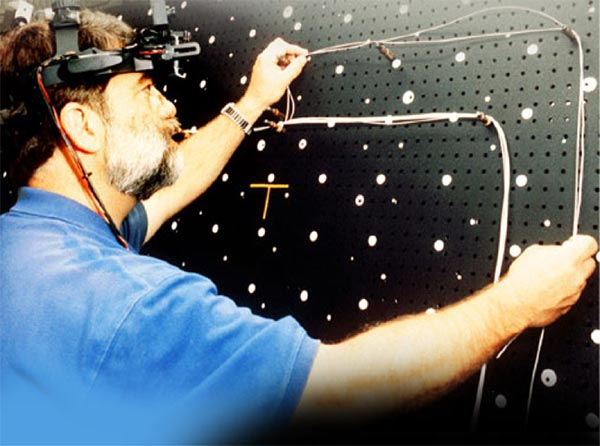
\includegraphics[width=\textwidth]{images/David-Mizell-AR.jpg}
    \caption{I ricercatori di Boeing hanno utilizzato un see-through HMD, creato da David Mizell, per guidare l'assemblaggio dei fasci di cavi per gli aerei.}
    \label{fig:figure12}
\end{figure}

Nel 1994 Paul Milgram pubblicò un articolo intitolato: “Augmented reality: A class of displays on the reality-virtuality continuum” \cite{Milgram}, introducendo i concetti di "reality-virtuality (RV) continuum" e di “mixed reality (MR)”, che definiscono la correlazione fra mondo reale e virtuale.

Negli anni successivi il campo della realtà aumentata ha continuato a evolversi e si è sempre più affermato nella cultura popolare. le tecnologie AR e VR sono diventate rapidamente di qualità superiore, più economiche e più ampiamente disponibili agli utenti.
\newpage
\section{Definizioni di VR, MR e AR}\label{sec:Sezione1.2}
Spesso i termini "realtà aumentata" e "realtà virtuale" vengono erroneamente interscambiati, quando in verità si tratta di due tecnologie con caratteristiche ben distinte.

Nella realtà aumentata le informazioni generate al computer vengono sovrapposte al mondo fisico, abbiamo quindi un mondo composto da una parte reale e una parte virtuale che sono in stretta correlazione fra loro. 

Entrando più nel dettaglio, gli aspetti chiave della realtà aumentata sono i seguenti:

\begin{itemize}
    \item Il mondo reale viene aumentato da informazioni digitali sovrapposte a esso.
    \item Le informazioni vengono visualizzate in registrazione spaziale e temporale con il mondo fisico.
    \item Le informazioni visualizzate dipendono dalla posizione e dalla prospettiva dell’utente nel mondo reale.
    \item L'esperienza di realtà aumentata è interattiva, ovvero l’utente può interagire con le informazioni e apportare modifiche a esse.
    \item Il livello d'interattività può variare dal semplice cambiamento della prospettiva alla manipolazione e persino alla creazione di nuove informazioni.
\end{itemize}

Nella realtà virtuale invece l’utente viene proiettato in un ambiente generato interamente al computer, non necessariamente correlato con il mondo reale.
I sensi vengono occlusi in tutto o in parte, in modo da far sembrare reale l’ambiente creato artificialmente.
Una volta definite le caratteristiche di queste due tecnologie la domanda che sorge spontanea è:
\begin{center}
"Che rapporto c’è fra VR e AR?"
\end{center}
La risposta la diede Paul Milgram nel 1994, pubblicando “Augmented Reality: A class of displays on the reality-virtuality continuum” \cite{Milgram} che, come detto nella sezione \ref{sec:Sezione1.1}, definisce i concetti di Reality-Virtuality Continuum e di Mixed Reality. 

Il RV continuum presenta una gamma di realtà che varia dal completamente reale al completamente virtuale (Figura \ref{fig:figure13}).
Secondo Milgram tutto ciò che risiede fra questi due estremi fa parte della Mixed Reality, che è composta dalla Augmented Reality, dove la realtà viene aumentata da entità virtuali e dalla Augmented Virtuality, dove il mondo virtuale viene aumentato da entità appartenenti al mondo reale.
\begin{figure}[t]
    \centering
    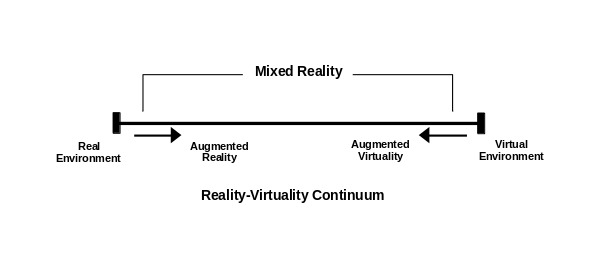
\includegraphics[width=\textwidth]{images/RV-continuum.jpg}
    \caption{Rappresentazione semplificata del Reality-Virtuality Continuum teorizzato da Paul Milgram.}
    \label{fig:figure13}
\end{figure}

Ciò che distingue la realtà mista da quella virtuale è l'integrazione delle entità virtuali nell'ambiente, chiamata registrazione spaziale; queste infatti, hanno una posizione e occupano uno spazio nel mondo fisico esattamente come se fossero reali, mentre nelle applicazioni AR il contenuto digitale si sovrappone al mondo reale senza integrarsi.
La Figura \ref{fig:figure14} descrive meglio questo concetto: abbiamo un’applicazione MR che introduce entità virtuali all’interno di un ambiente reale; 
la posizione di queste entità non dipende dalla posizione dell’utente nell’ambiente, quindi se ad esempio l’utente si spostasse verso un altro lato del tavolo vedrebbe la casa virtuale da un’altra prospettiva. 
Naturalmente è possibile anche interagire con le entità virtuali, che possono essere spostate, ridimensionate o anche eliminate.

\begin{figure}[t]
    \centering
    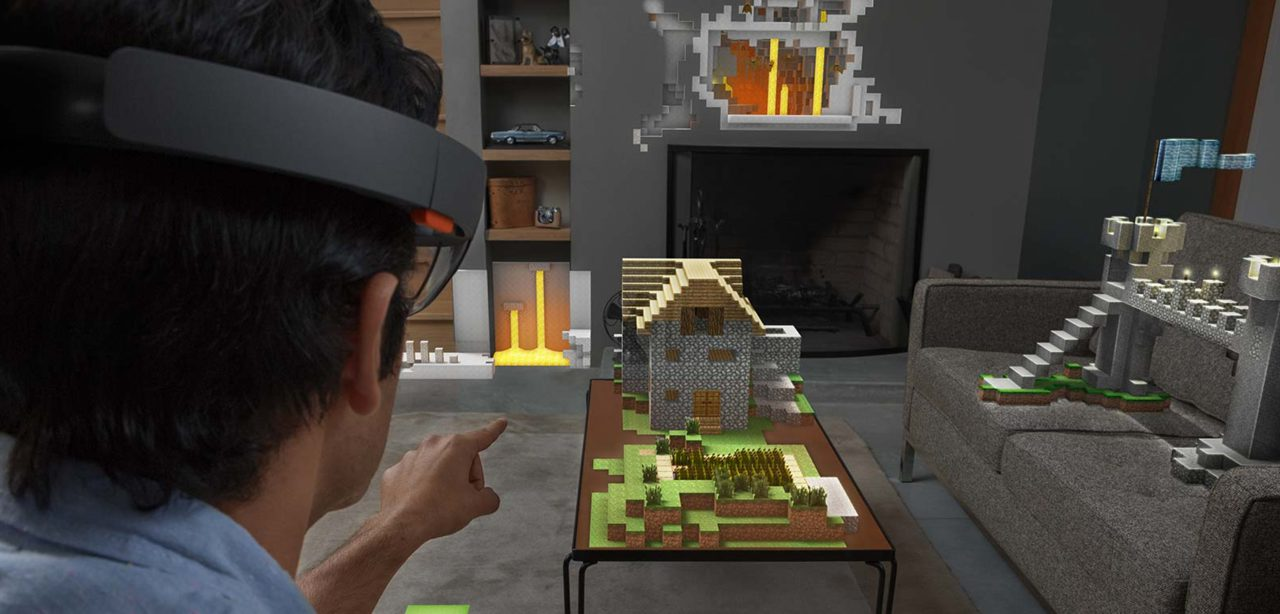
\includegraphics[width=\textwidth]{images/hololens-ar.jpg}
    \caption{Applicazione AR in cui le entità virtuali occupano una posizione nel mondo reale indipendentemente dalla collocazione e dai movimenti dell’utente.}
    \label{fig:figure14}
\end{figure}

In un certo senso, le entità digitali devono essere gestite come oggetti fisici almeno per quanto riguarda la questione della registrazione. Per questo motivo la registrazione con il mondo reale deve essere sia spaziale che temporale.

\section{Caratteristiche di un'Applicazione MR}\label{sec:Sezione1.3}
Nelle applicazioni MR le entità digitali vengono rappresentate dagli ologrammi (Figura \ref{fig:figure14}), che possono assumere qualsiasi forma ed emettere suoni. Inoltre, gli ologrammi possono modificare lo spazio fisico arricchendolo.

Ogni volta che un sistema software basato su AR deve aggiornare la vista dell'utente sull'ambiente Mixed Reality per mostrargli gli ologrammi, vengono richiesti due passaggi. Prima di tutto, il sistema deve identificare lo stato attuale del mondo fisico e calcolare di conseguenza lo stato del mondo digitale. In secondo luogo, emerge l'esigenza di visualizzare ologrammi in registrazione con la realtà in modo efficace considerando le percezioni umane. Generalmente lo stato in tempo reale del mondo fisico è ottenuto sfruttando i sensori forniti dal dispositivo, in particolare a questo scopo vengono utilizzate telecamere e tecniche di computer vision. Un problema significativo nella realtà aumentata è sapere dove si trova l'utente rispetto al sistema di riferimento del mondo reale, ovvero occuparsi del rilevamento del movimento e della posizione.

\subsection{Determinare la Posizione dell'Utente}
Nella realtà aumentata, determinare la prospettiva dell'utente significa calcolare la posa della telecamera, che è rappresentata da una posizione nello spazio 3D con sei gradi di libertà (6DOF). La posa si riferisce alla posizione e all'orientamento della fotocamera. Per identificare la posa della fotocamera è possibile utilizzare sensori inerziali (come accelerometro o giroscopio) e di posizione (come bussola o GPS). Una volta rilevata la posa della fotocamera, ovvero quando il sistema conosce la posizione e l'orientamento attuali dell'utente, gli ologrammi e i contenuti digitali possono essere presentati in allineamento con il mondo reale e proposti all'utente in un dato momento secondo la sua prospettiva. Secondo la letteratura, possono essere considerate diverse tecniche, eventualmente combinate, per determinare dove si trova l'utente e quale è il suo punto di vista. La tecnica più elementare, nota come AR marker based, dove il marker viene utilizzato per consentire il tracciamento al fine di determinare la posa del dispositivo. Oltre ai marker, possono essere applicate anche tecniche di tracciamento visivo in tempo reale. In particolare, il riferimento è a quelle tecniche che consentono una mappatura continua del mondo reale sfruttando un ampio insieme di punti rilevati, note anche come markerless AR.

Comunemente, un marker è un'immagine 2D asimmetrica che rappresenta un pattern molto semplice con l'obiettivo di essere rapidamente riconoscibile dagli algoritmi di visione artificiale (tipicamente modelli quadrati, in bianco e nero). In alcuni casi (ad esempio sfruttando Vuforia) è possibile sfruttare anche oggetti 3D come marker.
Grazie alla loro forma e struttura predefiniti, i marker possono essere localizzati facilmente dal visore. Quindi, vengono utilizzati per un rapido calcolo della posa.
Inoltre, per quanto riguarda quelli 2D, l'elevato contrasto dei quadrati in bianco e nero aiuta a facilitare il rilevamento.
I marker vengono posizionati nell'ambiente reale con lo scopo di individuare un sistema di riferimento da utilizzare per accoppiare il layer digitale con quello reale. Utilizzando un marker posto in una posizione ben nota del mondo reale, la funzione di tracciamento utilizza la fotocamera per stimare la posa del dispositivo in tempo reale in base a ciò che sta "vedendo". 

In condizioni di scarsa illuminazione o quando la telecamera è lontana dal marker tracciato, è possibile utilizzare tecniche basate sul rilevamento di \textit{natural feature point}.
Natural Feature Tracking (NFT) è una tecnica AR per riconoscere e tracciare una scena per determinare la posa della fotocamera, evitando deliberatamente di usare i marker.
NFT può sfruttare elementi incorporati nel mondo reale per migliorare i punti e le regioni di tracciamento. Il risultato può essere definito "markerless tracking" perché i "marker" non sono visibili all'utente.
Sebbene gli approcci senza marker possano sembrare la soluzione migliore, bisogna tenere in considerazione che tracciare la posa della fotocamera in ambienti sconosciuti può essere complicato. Negli ultimi anni è stata sviluppata una tecnologia nota come SLAM (Simultaneous Localization and Mapping), che ridefinisce l'idea originale di AR markerless basata su feature point. Tuttavia, l'NFT può essere meno costoso dal punto di vista computazionale di un sistema SLAM completo e generalmente è più adatto per i dispositivi mobili.
SLAM inizia con un ambiente sconosciuto e vuoto in cui il dispositivo di realtà aumentata cerca di generare una mappa e localizzarsi all'interno di essa. Attraverso una serie di algoritmi computazionalmente costosi, SLAM utilizza i dati del sensore IMU (unità di misura inerziale) per costruire una mappa dell'ambiente sconosciuto e allo stesso tempo per identificare la sua posizione.
Infine, l'AR markerless utilizza in genere anche la funzione GPS per tracciare la posizione dell'utente in scenari all'aperto combinata con il tracciamento visivo per ottenere l'orientamento correlato. 

\subsection{Sistemi di Coordinate}
Per familiarità, accuratezza e semplicità, la maggior parte degli ambienti virtuali è definita utilizzando un sistema di coordinate cartesiane standard, come mostrato in Figura \ref{fig:figure15}. All'interno di questo sistema, ogni punto è specificato in modo univoco utilizzando tre coordinate numeriche (x, y, z) che rappresentano distanze specifiche (misurate nella stessa unità di lunghezza) da tre piani reciprocamente perpendicolari. 

Oltre a essere l'approccio più comunemente utilizzato per la mappatura di spazi reali e virtuali, il sistema cartesiano viene impiegato anche per definire la posizione e il punto di vista di un utente nello spazio.

\begin{figure}[H]
    \centering
    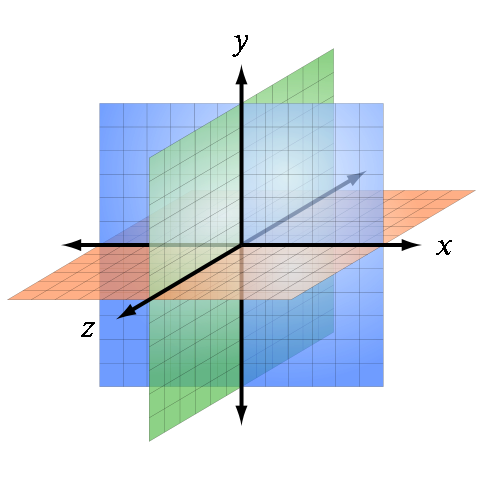
\includegraphics[width=0.6\textwidth]{images/sistema-cartesiano.png}
    \caption{Ogni punto nel sistema di coordinate cartesiane 3D è identificato in modo univoco da valori x, y e z.}
    \label{fig:figure15}
\end{figure}

Un ologramma posto in un ambiente tridimensionale deve avere l'abilità di muoversi liberamente e di ruotare sui tre assi perpendicolari.
Poiché il movimento lungo ognuno degli assi è indipendente quanto per gli assi di traslazione che per gli assi di rotazione, il movimento ha quindi sei gradi di libertà (6DoF: Six Degrees Of Freedom).
Per garantire questa caratteristica è possibile sfruttare gli angoli di Eulero o i quaternioni.
Solitamente vengono utilizzati i quaternioni perché con gli angoli di Eulero può presentarsi il fenomeno del blocco cardanico (in inglese gimbal lock), che avviene quando vengono allineati i due assi rotanti verso la stessa direzione, causando la perdita di un grado di libertà sull'asse bloccato.

\subsection{Interazioni con gli Ologrammi}
La realtà aumentata è, per sua natura, un mezzo interattivo. Se il contenuto digitale deve essere percepito come parte del mondo reale, poiché le persone possono interagire con oggetti fisici anche nei sistemi AR gli utenti dovrebbero essere in grado di interagire con gli ologrammi in modo simile. In effetti, l'interazione gioca un ruolo chiave nell'esperienza complessiva dell'utente. In un ambiente AR, l'interazione è generalmente limitata all'azione da eseguire sugli elementi digitali, ad esempio osservarli o afferrarli e spostarli da una posizione a un'altra. L'interazione in AR è un aspetto che dipende principalmente dal dispositivo utilizzato per tracciare e mostrare ologrammi nell'ambiente Mixed Reality. La capacità di interagire con gli ologrammi aumenta proporzionalmente e diventa più potente in relazione all'efficienza del dispositivo AR utilizzato in termini di propri sensori e capacità computazionali. 

\subsection{Esperienze Multi-Utente}
Il mondo reale è un ambiente cooperativo multiutente, gli ambienti di realtà mista diventano più interessanti quando anche il livello digitale e gli ologrammi possono essere condivisi tra più utenti che interagiscono contemporaneamente. Proporre un'esperienza multiutente cooperativa significa avere un layer digitale condiviso in tempo reale. Prima di tutto, gli utenti dovrebbero essere in grado di osservare gli stessi ologrammi ma dalla propria prospettiva. In questo caso, utilizzando dei marker, questa caratteristica potrebbe essere semplicemente ottenuta, ad esempio, con due utenti che osservano contemporaneamente lo stesso marker che propone per entrambi gli stessi sistemi di riferimento e orientamento. Sfortunatamente, questa è una soluzione che nasconde il vero problema: in questo caso, lo stato dell'ologramma non è realmente condiviso tra gli utenti. Ad esempio, se un utente sposta l'ologramma, l'altro utente continuerà a vedere l'ologramma nella posizione originale. Per risolvere i problemi proposti c'è l'esigenza che entrambi gli utenti facciano riferimento alla stessa istanza dell'ologramma osservato da entrambi, una sorta di centralizzazione dell'istanza del livello digitale, a cui accedono più utenti. Non sorprende che per sperimentare un ambiente MR multiutente cooperativo completo emergano esigenze che sono ben lungi dall'essere affrontate dalle soluzioni infrastrutturali software attualmente disponibili. Soprattutto quando la cooperazione non è intesa solo tra umani ma coinvolge anche entità software autonome e altre cose fisiche appartenenti al mondo reale.
Un altro problema è dato dai diversi dispositivi che si possono usare per accedere all'esperienza condivisa. Con dispositivi (ad esempio smartphone e visori) basati su piattaforme differenti (come Windows, Lumin OS, Android e iOS) sorge l'esigenza di sviluppare API comuni per garantire l'interoperabilità delle applicazioni MR indipendentemente dalla piattaforma che si sta utilizzando.
Una delle soluzioni proposte per venire a capo di questo problema è OpenXR, ovvero un'API che si occupa di fornire un accesso nativo alle piattaforme e ai dispositivi di
Augmented, Mixed e Virtual Reality.

\section{Tassonomia dei Dispositivi MR}\label{sec:Sezione1.4}
Al giorno d’oggi è disponibile una moltitudine di dispositivi MR, che si contraddistinguono in base ai sistemi di input, output ed elaborazione che utilizzano. 

In generale, è possibile identificare due macrocategorie di sistemi AR: wearable (indossabili) e non-wearable (non indossabili). 

Un’altra suddivisione può essere fatta distinguendo i dispositivi che sono stati concepiti appositamente per esperienze MR da quelli più generici (come PC e smartphone).

Alcuni dispositivi, come le lenti a contatto per la realtà aumentata, sono ancora in fase di sviluppo e non sono ancora disponibili prodotti commerciali.

\subsection{Head Mounted Display}
Un head mounted display è un visore incorporato in un casco, dotato di dispositivi di registrazione dell'orientamento per il movimento sincronizzato della testa e degli occhi dell’utente.
Esistono due tipi di HMD attualmente in commercio, quelli che supportano esclusivamente esperienze VR (HTC Vive e Oculus Rift, Figura \ref{fig:figure16}) e quelli progettati per esperienze AR (come HoloLens 2 e Magic Leap 1, Figura \ref{fig:figure17}).

\begin{figure}[H]
    \centering
    \begin{subfigure}[b]{0.4\textwidth}
        \centering
        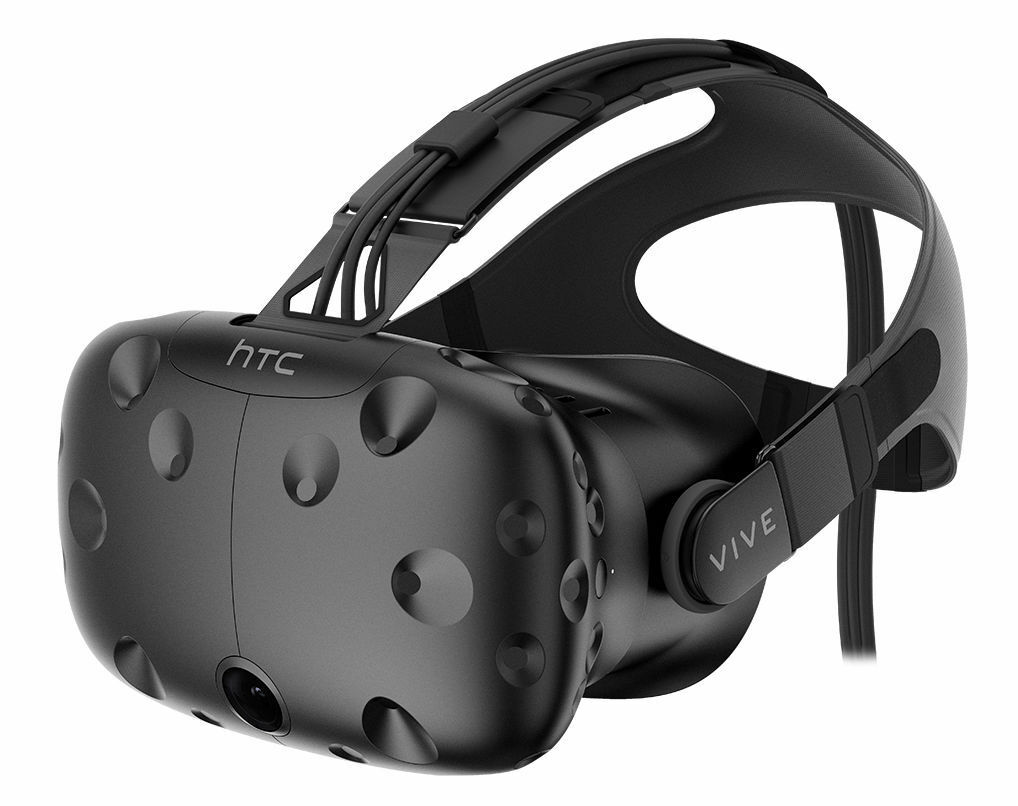
\includegraphics[width=\textwidth]{images/HTC-Vive.JPG}
        \caption{HTC Vive}
        \label{fig:figure16a}
    \end{subfigure}
    \begin{subfigure}[b]{0.4\textwidth}
        \centering
        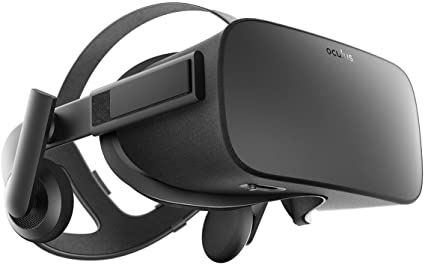
\includegraphics[width=\textwidth]{images/Oculus-Rift.jpg}
        \caption{Oculus Rift}
        \label{fig:figure16b}
    \end{subfigure}
       \caption{HTC Vive e Oculus Rift messi a confronto}
       \label{fig:figure16}
\end{figure}

Rift utilizza un singolo sensore esterno, un cilindro nero che si trova su un supporto da tavolo in metallo alto 23 centimetri. Il sensore può inclinarsi verso l'alto e verso il basso e deve essere posizionato in un punto in cui possa mantenere una visione chiara del visore quando è in uso. Un secondo sensore identico traccia i controller Oculus Touch, questi due sensori inoltre lavorano in tandem per migliorare il tracciamento di tutti i dispositivi e coprire un'area più ampia rispetto alla posizione fissa consentita da un solo sensore. 

HTC Vive è composto non solo da un visore per la realtà virtuale e da due sofisticati controller, ma anche da un sistema di due telecamere laser (base station) che hanno il compito di tracciare il movimento dell'utente all’interno della stanza. HTC Vive supporta un’area che può avere una dimensione massima di cinque metri di diagonale, pari alla massima distanza consigliata per le due base station, sufficiente per coprire interamente una stanza di circa 12 metri quadri, e dare così l’impressione di potersi muovere liberamente nel mondo virtuale.

Gli HMD che supportano la realtà aumentata sfruttano una tecnologia definita \textit{optical see-through}, che permette di vedere attraverso il display.

Magic Leap 1 è dotato di uno schermo LCOS prodotto da Omnivision, che offre una definizione di 1280 x 960. Mentre il primo HoloLens aveva uno schermo con definizione HD (720p) e un campo visivo di 30 gradi, il suo successore è stato migliorato notevolmente e infatti ha un campo visivo di 52 gradi. HoloLens 2 supera Magic Leap in termini di definizione con il suo schermo che offre una definizione di circa 2K per occhio. In totale, questo nuovo visore visualizza 47 pixel per grado. Lo schermo di HoloLens 2 è quindi superiore in termini di definizione, mentre i due visori AR sono uguali in termini di campo visivo.

\begin{figure}[t]
    \centering
    \begin{subfigure}[b]{0.4\textwidth}
        \centering
        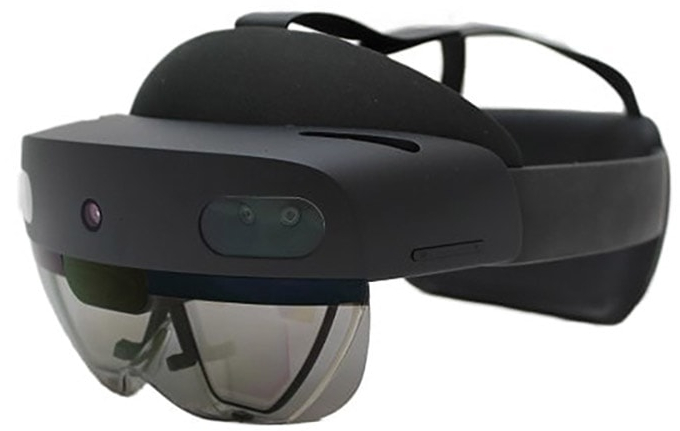
\includegraphics[width=\textwidth]{images/Hololens2.jpg}
        \caption{Microsoft HoloLens 2}
        \label{fig:figure17a}
    \end{subfigure}
    \begin{subfigure}[b]{0.55\textwidth}
        \centering
        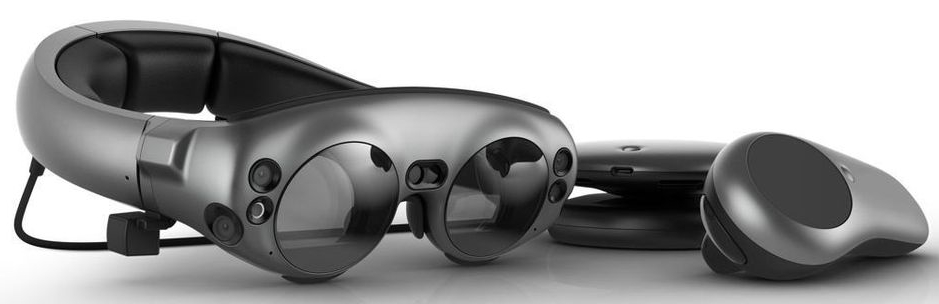
\includegraphics[width=\textwidth]{images/Magic-Leap1.jpg}
        \caption{Magic Leap 1}
        \label{fig:figure17b}
    \end{subfigure}
       \caption{HoloLens 2 e Magic Leap 1 messi a confronto}
       \label{fig:figure17}
\end{figure}

Magic Leap 1 viene fornito con il suo controller "Control". Questo controller offre sei gradi di libertà di movimento senza la necessità di sensori esterni aggiuntivi. Si basa sul tracciamento del campo elettromagnetico. È questo accessorio, simile ai controller per visori VR Oculus Rift o HTC Vive, che permette di interagire nella realtà aumentata di Magic Leap.
Magic Leap 1 offre anche funzioni di tracciamento dell'iride e della mano. Quest'ultimo punto permette di interagire usando le mani in modo naturale. In realtà, questo sistema non rileva la posizione delle dita dell'utente nello spazio, ma solo gesture predefinite.
HoloLens 2 si distingue per una tecnologia di tracciamento della mano decisamente accurata. Infatti, questo nuovo visore AR è in grado di seguire la posizione delle dieci dita dell'utente. Pertanto, è persino possibile suonare il pianoforte in realtà aumentata.
Come con il primo HoloLens, purtroppo, è ancora necessario che le mani rimangano nel campo visivo di HoloLens 2 per il tracciamento.
Troviamo anche la stessa tecnologia di eye tracking degli smartphone Lumia. L'Eye Tracking di HoloLens 2 è molto più avanzato, incluso lo sblocco del dispositivo sfruttando l'iride con Windows Hello. Anche il riconoscimento vocale è stato migliorato e ora è possibile controllare il dispositivo sfruttando i comandi vocali.

\subsection{Head-up Display}
Gli head-up display (Figura \ref{fig:figure18}) sono stati sviluppati inizialmente per essere adottati in ambito militare, in particolare per proiettare informazioni utili nel campo visivo dei piloti di aerei.
Successivamente gli HUD sono stati impiegati anche nel settore commerciale, ad esempio nelle auto vengono utilizzati per rendere immediatamente disponibili alcuni dati utili alla guida, senza che il guidatore debba distogliere lo sguardo dalla strada per concentrarsi sul quadro strumenti.
\begin{figure}[H]
    \centering
    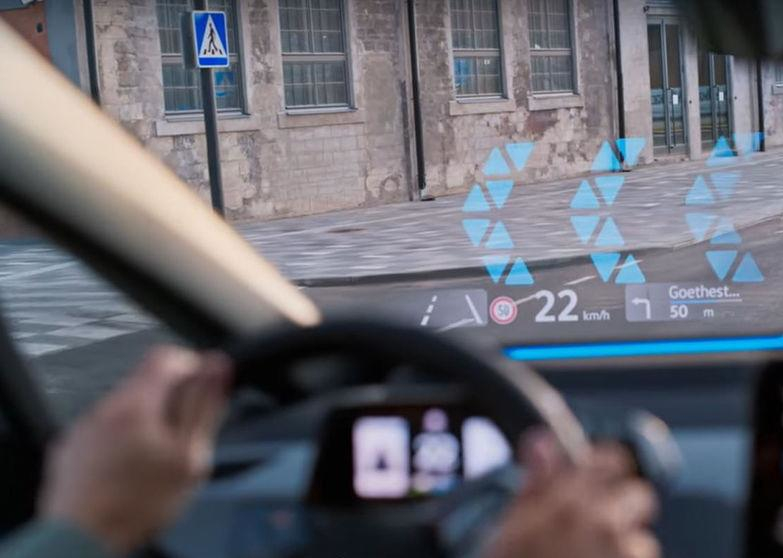
\includegraphics[width=0.8\textwidth]{images/Augmented-Reality-Head-Up-Display.jpg}
    \caption{Head-up Display.}
    \label{fig:figure18}
\end{figure}
\newpage
\subsection{Smart-Glasses}
Gli smart-glasses (Figura \ref{fig:figure19}) sono occhiali che permettono all’utente di ricevere informazioni direttamente sulle lenti.
I primi modelli potevano eseguire solo attività base, delegando il carico computazionale a dispositivi mobili come smartphone e tablet, connessi tramite Bluetooth, oggi invece sono in grado di eseguire vere e proprie applicazioni autonomamente.

\begin{figure}[H]
    \centering
    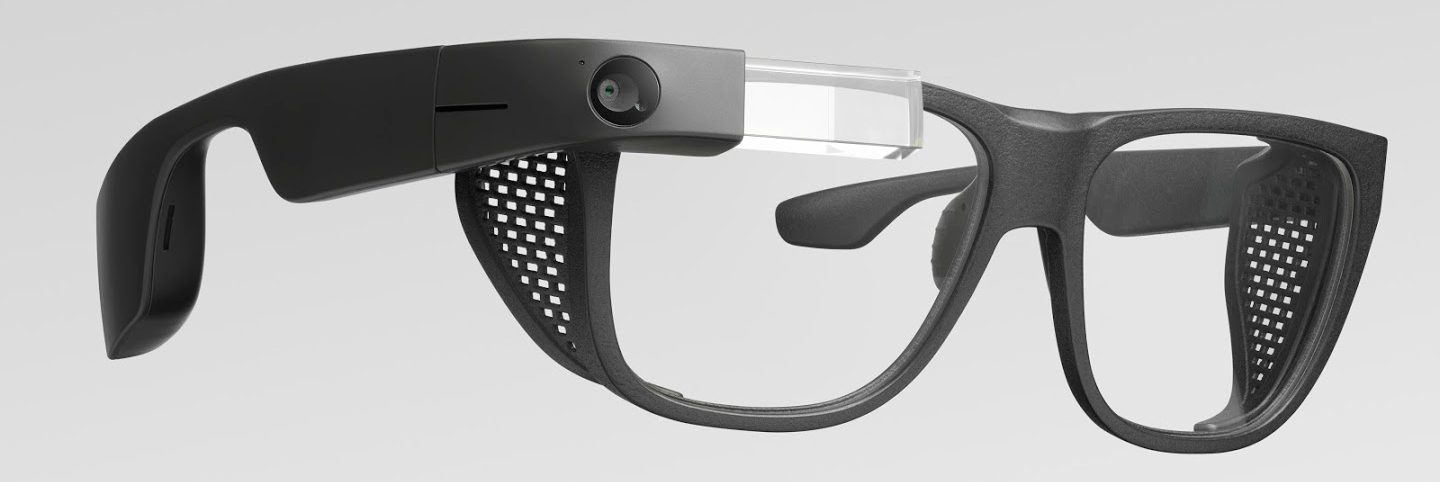
\includegraphics[width=0.7\textwidth]{images/smart-glass.jpg}
    \caption{Google Glass.}
    \label{fig:figure19}
\end{figure}

\subsection{Dispositivi Mobili}
La categoria dei dispositivi mobili riguarda device come smartphone e tablet che eseguono Android o iOS.
Questi apparati non sono stati progettati appositamente per esperienze AR, tuttavia negli ultimi anni sono state sviluppate piattaforme come Google ARCore e Apple ARKit, che rendono possibile lo sviluppo di applicazioni AR sfruttando la sensoristica dei device.

I dispositivi mobile sfruttano una tecnologia di tipo \textit{video see-through}.
La videocamera cattura il mondo reale dal punto di vista dell’utente, in fase di elaborazione vengono aggiunte le informazioni digitali e infine il risultato viene riportato sul display del device (Figura \ref{fig:figure110}).
\begin{figure}[H]
    \centering
    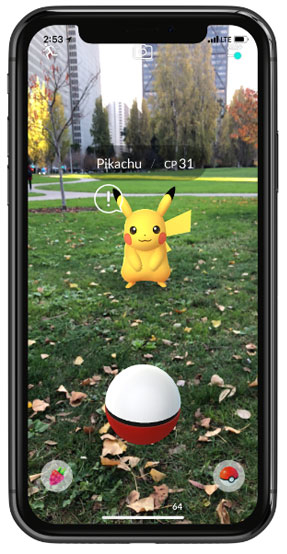
\includegraphics[scale=0.5]{images/pokemon_go.jpg}
    \caption{Applicazione AR in esecuzione su un dispositivo mobile.}
    \label{fig:figure110}
\end{figure}

\section{Framework di Sviluppo MR}\label{sec:Sezione1.5}
Per realizzare applicazioni MR è necessario considerare le piattaforme e i dispositivi di destinazione, questo perché oggi sono disponibili vari framework di sviluppo, realizzati per piattaforme specifiche o per garantire l'interoperabilità fra i diversi sistemi attualmente in commercio.

\subsection{Microsoft Mixed Reality Toolkit}
Mixed Reality Toolkit (MRTK) \footnote{https://github.com/Microsoft/MixedRealityToolkit-Unity} è un progetto gestito da Microsoft che fornisce un set di componenti e funzionalità che consentono lo sviluppo di app di realtà mista multipiattaforma.
Per sfruttare le funzionalità offerte da questo framework è necessario integrarlo in ambienti di sviluppo come Unity o Unreal Engine.
MRTK è modulare, questo significa che è possibile installare nell'ambiente di sviluppo solo i componenti necessari per lo sviluppo dell’applicazione; in questo modo la dimensione del progetto rimane contenuta. Inoltre, poiché è costruito con oggetti scriptabili, è anche possibile sostituire i componenti inclusi con i propri, per supportare altri servizi, sistemi e piattaforme. 
MRTK è in continuo sviluppo, vengono introdotte nuove funzionalità e risolti problemi costantemente, allo stesso tempo alcune funzionalità vengono deprecate.
MRTK viene impiegato nello sviluppo di applicazioni AR per HoloLens 1 e 2.

\subsection{Apple ARKit}
ARKit \footnote{https://developer.apple.com/augmented-reality/arkit/} è la piattaforma di realtà aumentata (AR) di Apple per dispositivi iOS.
Questa piattaforma di sviluppo che consente agli sviluppatori di app di creare rapidamente e facilmente esperienze AR nelle loro app e giochi. Utilizza la fotocamera, i processori e i sensori di movimento del dispositivo per creare interazioni coinvolgenti.

Per creare una corrispondenza tra spazio reale e virtuale, ARKit utilizza una tecnica chiamata Visual Inertial Odometry. Questo processo combina le informazioni provenienti dall'hardware di rilevamento del movimento del dispositivo iOS con l'analisi della visione artificiale della scena visibile dalla fotocamera del dispositivo. ARKit riconosce i feature point nell'immagine della scena, tiene traccia delle differenze nelle posizioni di tali punti tra i fotogrammi video e confronta tali informazioni con i dati di rilevamento del movimento. Il risultato è un modello ad alta precisione della posizione e del movimento del dispositivo.

Il monitoraggio del mondo analizza e comprende anche i contenuti di una scena. Vengono utilizzati metodi di ray-casting per trovare superfici del mondo reale corrispondenti a un punto nell'immagine della telecamera. Abilitando l'impostazione planeDetection nella configurazione della sessione, ARKit rileva le superfici piane nell'immagine della telecamera e ne riporta la posizione e le dimensioni. È anche possibile utilizzare i risultati ray-cast o i piani rilevati per posizionare o interagire con il contenuto virtuale nella scena. 

\subsection{Google ARCore}
ARCore \footnote{https://developers.google.com/ar/} è un framework di sviluppo software sviluppato da Google che consente di creare applicazioni di realtà aumentata.
La tecnologia di tracciamento del movimento di ARCore utilizza la fotocamera del telefono per identificare i feature point e tiene traccia di come questi punti si muovono nel tempo. Con una combinazione del movimento di questi punti e delle letture dei sensori inerziali del telefono, ARCore determina sia la posizione che l'orientamento del telefono mentre si muove nello spazio.

Oltre a identificare i punti chiave, ARCore può rilevare superfici piane, come un tavolo o il pavimento, e può anche stimare l'illuminazione media nell'area circostante. Queste capacità si combinano per consentire ad ARCore di costruire la propria comprensione del mondo che lo circonda.

La comprensione di ARCore del mondo reale consente di posizionare oggetti, annotazioni o altre informazioni in un modo che si integra perfettamente con il mondo reale.
Grazie al rilevamento del movimento l'utente può spostarsi e visualizzare gli oggetti virtuali da qualsiasi angolazione.

ARCore fornisce SDK per molti degli ambienti di sviluppo più diffusi. Questi SDK forniscono API native per tutte le funzionalità AR essenziali come il rilevamento del movimento, la comprensione dell'ambiente e la stima della luminosità. Con queste funzionalità è possibile creare esperienze AR completamente nuove o migliorare le app esistenti con funzionalità AR.

\subsection{OpenXR}
OpenXR \footnote{https://www.khronos.org/OpenXR/} è un’Application Program Interface (API), ad alte prestazioni, royalty-free (licenza che permette all'utente di utilizzare la risorsa senza limiti di tempo e spazio senza dover sostenere ulteriori costi) sviluppata da Khronos, la quale si occupa di fornire un accesso nativo alle piattaforme e ai dispositivi di Augmented, Mixed e Virtual Reality. Il termine XR, infatti, sta per eXtended Reality e comprende descritte nella sezione \ref{sec:Sezione1.2}.
OpenXR dal punto di vista del programmatore, consiste in un insieme di funzioni che si interfacciano con una runtime, per eseguire operazioni comunemente richieste come ad esempio: accedere al controller o allo stato della periferica utilizzata, ottenere le posizioni di tracciamento dei dispositivi di input o della testa dell’utente e inviare frame renderizzati.

OpenXR mira a semplificare lo sviluppo del software AR/VR, consentendo alle applicazioni di raggiungere una gamma più ampia di piattaforme hardware senza dover trasferire o riscrivere il codice e, successivamente, consentendo ai fornitori di piattaforme che supportano OpenXR di accedere a più applicazioni.

Senza uno standard multipiattaforma, le applicazioni e gli engine VR/AR devono utilizzare le API proprietarie di ciascuna piattaforma. I nuovi dispositivi di input richiedono l'integrazione di driver personalizzati (Figura \ref{fig:figure111a}).

OpenXR fornisce accesso multipiattaforma e ad alte prestazioni direttamente alle diverse runtime dei dispositivi XR su più piattaforme. OpenXR consente l'esecuzione di applicazioni ed engine, incluso WebXR, su qualsiasi sistema che esponga le API OpenXR (Figura \ref{fig:figure111b}).

\begin{figure}[t]
    \centering
    \begin{subfigure}{0.6\textwidth}
        \centering
        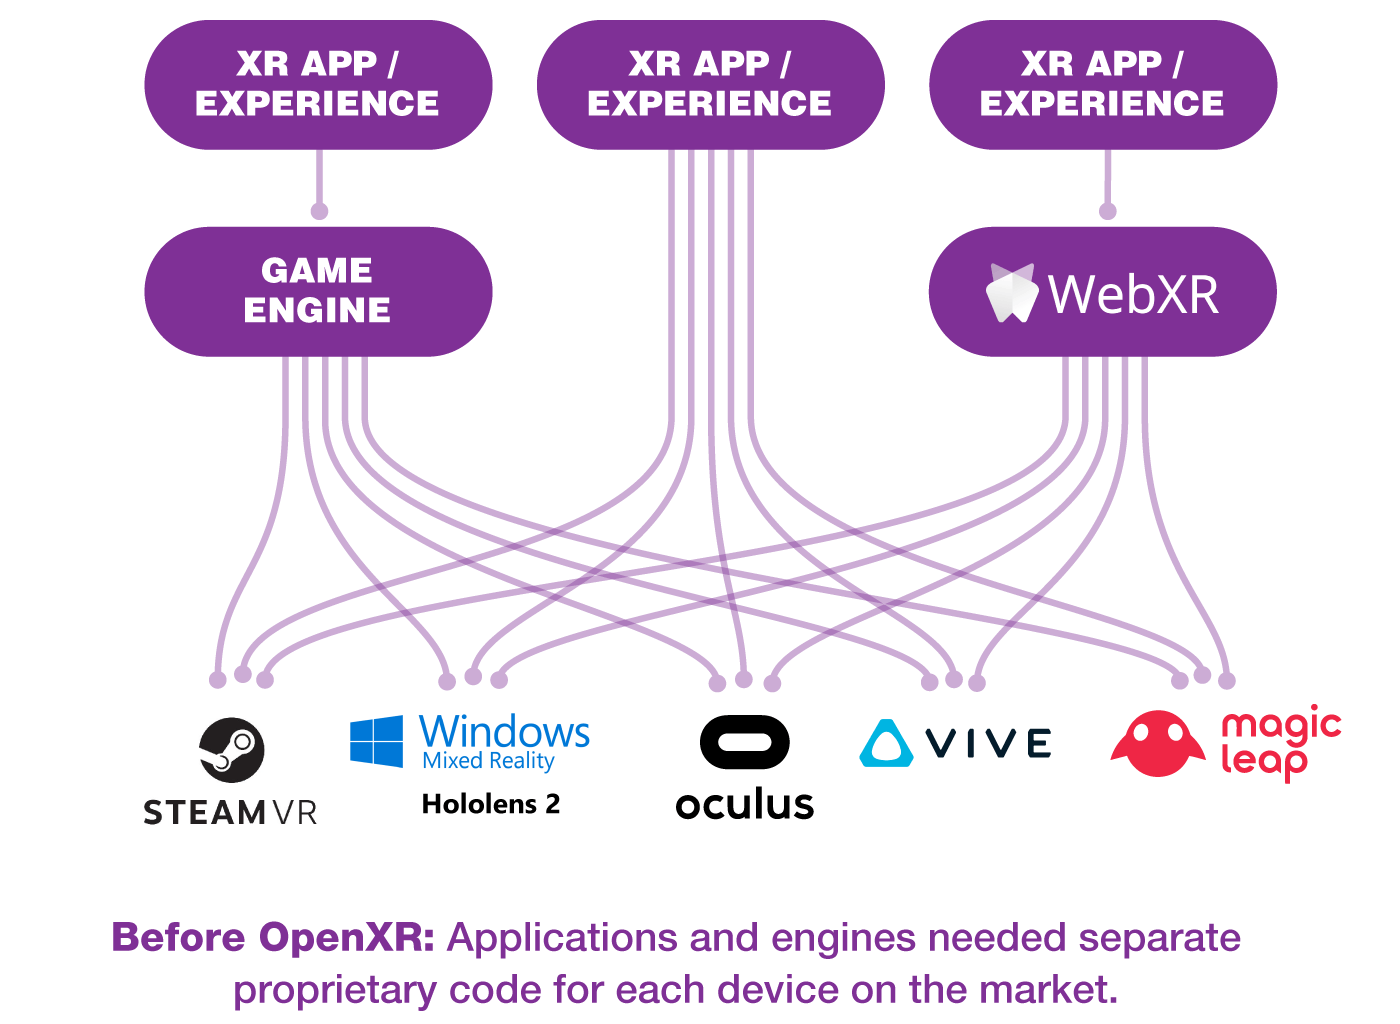
\includegraphics[width=\textwidth]{images/OpenXR-Before_3.png}
        \caption{Sviluppo senza OpenXR}
        \label{fig:figure111a}
    \end{subfigure}
    \begin{subfigure}{0.6\textwidth}
        \centering
        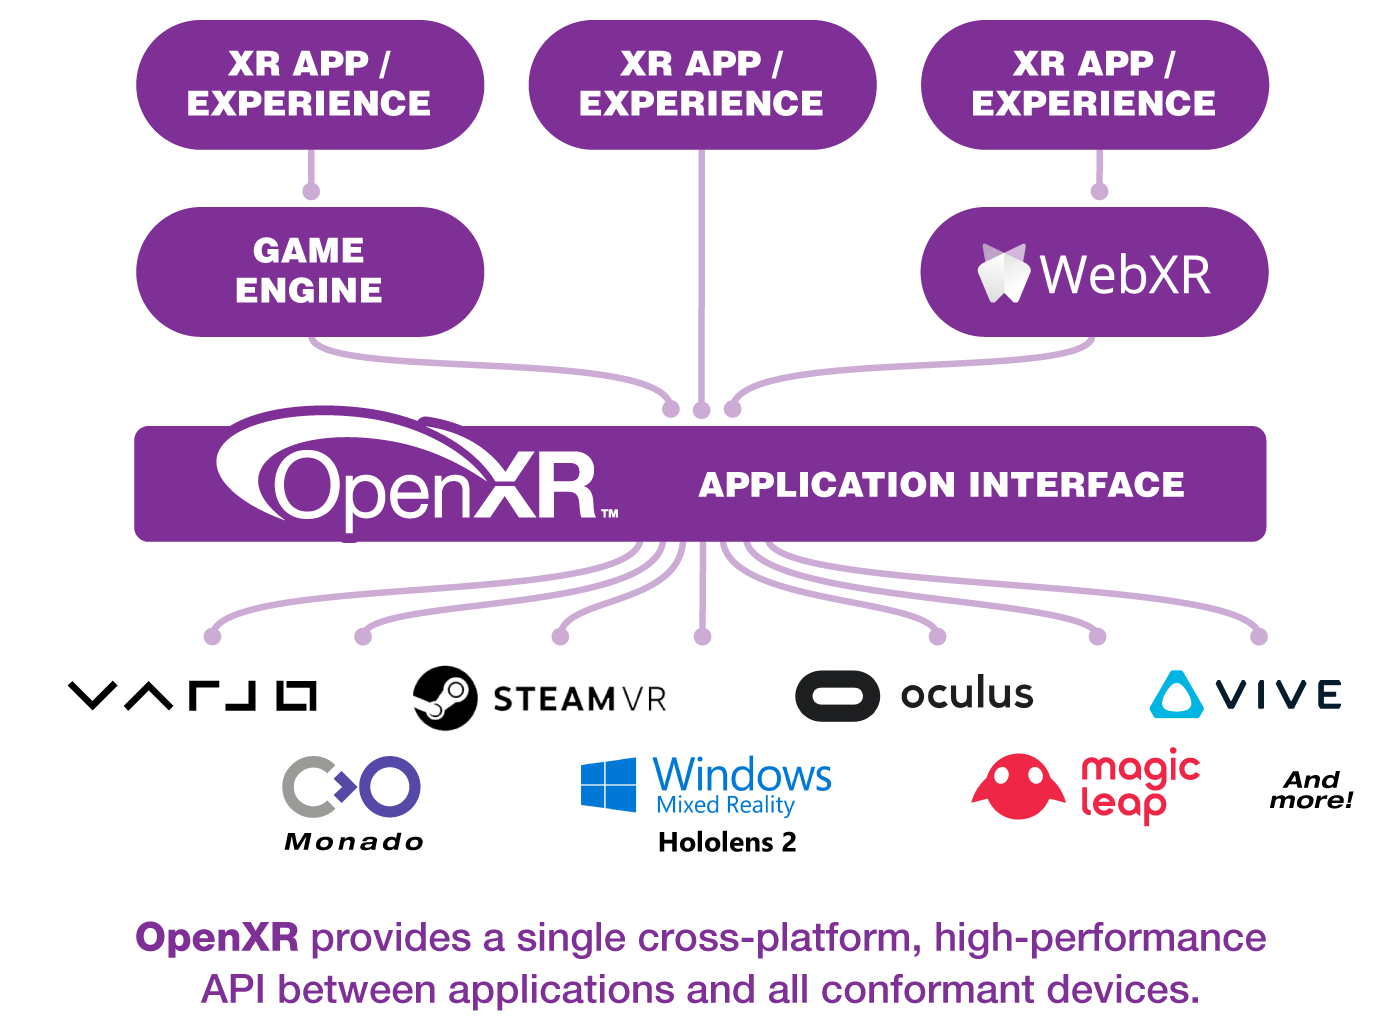
\includegraphics[width=\textwidth]{images/OpenXR-After_3.png}
        \caption{Sviluppo con OpenXR}
        \label{fig:figure111b}
    \end{subfigure}
       \caption{Problema della frammentazione risolto da OpenXR}
       \label{fig:figure111}
\end{figure}

\subsection{Vuforia}
Vuforia \footnote{https://developer.vuforia.com/} è un framework di sviluppo per applicazioni AR ed è stato introdotto da Qualcomm, un'azienda inizialmente specializzata nella ricerca e nello sviluppo dei mezzi di comunicazione wireless e dei microchip elettronici SoC.

Nel cuore della piattaforma si trova una libreria QCAR scritta in C++, che supporta vari tipi di target (image cube, cuboid, cylinder, word target e frame marker) e funzionalità di rendering dell'immagine. I target in Vuforia sono, fondamentalmente, oggetti reali, che possono essere sfruttati dalla applicazione per posizionare oggetti virtuali o per condividere sistemi di coordinate con altri dispositivi.

Vuforia dispone anche di Extended Tracking: dopo il primo rilevamento il dispositivo mantiene il tracciamento anche quando il target non è più visibile, quindi una volta trovato il target l’utente è libero di muoversi nell’ambiente.

Quella che segue è una descrizione di alto livello del processo di rilevazione del target: 
\begin{enumerate}
\item Il Tracker di Vuforia Engine riconosce il target.
\item Il tracciamento del target viene quindi inizializzato. 
\item La posizione e la rotazione del target vengono analizzate per fornire una stima della posa al dispositivo. 
\item Vuforia Engine trasforma la posa del target nel sistema di coordinate del dispositivo. 
\item Il dispositivo assume il controllo nel momento in cui il target non è più visibile.
Quando il target compare nuovamente nel campo visivo Vuforia esegue nuovamente il tracciamento. 
\end{enumerate}
